\documentclass[12pt,letterpaper]{article}

% \input{worksheet-setup.tex}
\usepackage{fancyhdr,fancybox}
\usepackage{amsmath}
\usepackage{amsthm}
\usepackage{amssymb}
\usepackage{tikz}

\usepackage{enumitem}
\usepackage{multicol}

%%
%% Page set-up:
%%
\pagestyle{empty}
\lhead{\textsc{3B - Derivatives Review}} %=================UPDATE THIS=================%
\rhead{\textsc{Fall 2019}}
%\chead{\Large\textbf{A New Integration Technique \\ }}
\rfoot{trevorklar@math.ucsb.edu}
\renewcommand{\headrulewidth}{1pt}

\setlength{\parindent}{0in}
\setlength{\textwidth}{7in}
\setlength{\evensidemargin}{-0.25in}
\setlength{\oddsidemargin}{-0.25in}
\setlength{\parskip}{.5\baselineskip}
\setlength{\topmargin}{-0.5in}
\setlength{\textheight}{9in}

\setlist[enumerate,1]{label=\textbf{\arabic*.}}

\begin{document}
\thispagestyle{fancy}
\begin{center}
3B - Integral Calculus \\
Week 1 %=================UPDATE THIS=================%
\end{center}

\hrule

\begin{center}
\begin{tabular}{|rl|}
\hline
\multicolumn{2}{|c|}{Contact Information} \\
\hline
\bf{TA's name:} & Trevor Klar \\
\bf{Email:} & trevorklar@math.ucsb.edu \\
\bf{Office hours:} & Mondays 2:00-3:00 \\
\bf{Math Lab hours:} & Wednesdays 12:00-2:00 \\
\bf{Office:} & South Hall 6431x \\
\hline
\end{tabular}
\end{center}

 %=================START OF WORKSHEET=================%

In this course we're going to do a \emph{lot} of integration, and once you learn how to do them, you'll find that they involve a lot of doing derivatives-- backwards. So let's see how well we remember our derivatives from 3A:
\bigskip


Find the following anti-derivatives using this idea.
\begin{multicols}{2}
  \begin{enumerate}[series=problems]
  \item $\displaystyle\int \arctan(x)\,dx$

  \item $\displaystyle \int x^2 \ln(x) \, dx$
  \end{enumerate}
\end{multicols}
\vfill

\begin{multicols}{2}
  \begin{enumerate}[resume=problems]
  \item $\displaystyle \int \ln(x) \, dx$

  \item $\displaystyle \int x^k \ln(x) \, dx$
  \end{enumerate}
\end{multicols}
\vfill

\begin{multicols}{2}
  \begin{enumerate}[resume=problems]
  \item $\displaystyle\int x e^{2x}\,dx$

  \item $\displaystyle \int x^2 e^{kx} \, dx$

  \end{enumerate}
\end{multicols}
\vfill

\newpage

\begin{multicols}{2}
  \begin{enumerate}[resume=problems]
  \item $\displaystyle \int x^3 e^{2x^2}\, dx$

  \item $\displaystyle \int x\sin(x)\, dx$

  \end{enumerate}  
\end{multicols}
\vfill

\begin{enumerate}[resume=problems]
\item Find $\displaystyle\int_0^1 \arcsin(x)\, dx$ in two ways:

\begin{minipage}{0.6\linewidth}
  \begin{enumerate}[series=part]
    \item Find the shaded region to the right by writing it as a
    ``$dy$'' integral.  What does this have to do with the given integral?
    \vspace*{2in}
    
  \end{enumerate}
\end{minipage}
\hfill
\begin{minipage}{0.35\linewidth}
  \begin{tikzpicture}[x=30mm,y=20mm,>=latex]
    \draw[thick,black,->] (0,0) -- (1.2,0) node[below] {$x$};
    \draw[thick,black,->] (0,0) -- (0,2) node[left] {$y$};
    % ticks:
    \foreach \x in {0,1} \draw[thin,black] (\x,0) -- (\x,-2pt) node[below] {$\x$};
    \foreach \y in {0} \draw[thin,black] (0,\y) -- (-2pt,\y) node[left] {$\y$};
    \draw[thin,black] (0,{pi/2}) -- (-2pt,{pi/2}) node[left] {$\frac{\pi}{2}$};
    \draw[ultra thick,black] plot[domain=0:2,samples=200] ({sin(\x r)},\x);
    \node[above right] at (1,{pi/2}) {$y=\arcsin(x)$};
    \draw[thick,black,fill=gray!20] plot[domain=0:{pi/2},samples=200] ({sin(\x r)},\x) -- (0,{pi/2}) -- cycle;
  \end{tikzpicture}
\end{minipage}
\begin{enumerate}[resume=part]
\item Use the trick we've worked on today.
  \vfill
\end{enumerate}
\end{enumerate}


\end{document}


%%% Local Variables: 
%%% mode: latex
%%% TeX-master: t
%%% End: 
